\documentclass[a4paper]{article}

\usepackage{times}
\usepackage[ngerman]{babel}
\usepackage[T1]{fontenc}
\usepackage{amsmath}
\usepackage{amsfonts}
\usepackage{graphicx}
\usepackage{authblk}
\usepackage{fancyhdr}

\pagestyle{fancy}
\renewcommand{\headrulewidth}{0,6pt}
\fancyhead[L]{\leftmark}
\fancyhead[R]{\thepage}

\title{\Huge{Elektrik\\Lernzettel}}
\date{\today}
\author{\quad\\Baden, Julian\\Hagemann, Florian\\\quad\\Gymnasium Mellendorf\\ABI Jahr 2027}


\begin{document}

\maketitle
\thispagestyle{empty}
\newpage
\tableofcontents \thispagestyle{empty}
\newpage
\pagenumbering{arabic}

%________________________________________________________________________________________________

\section{Formelsammlung}
\subsection{Einheiten}



\newpage


\section{Magnetische Felder}
Der Magnetismus ist eine physikalische Erscheinung, die sich unter anderem als Kraft\-wirkung zwischen Magneten, magnetisierten bzw. magnetisierbaren Gegenständen und bewegten elektrischen Ladungen äußert. Er lässt sich beschreiben durch ein Magnetfeld, das einerseits von diesen Objekten erzeugt wird und andererseits auf sie wirkt. 
Die Magnetfeldlinien gehen immer vom Nord- zum Südpol.

\begin{figure}[h]
    \centering
    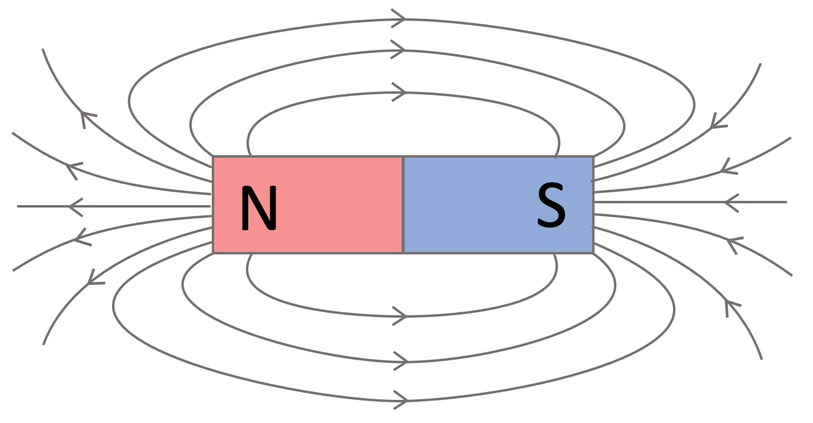
\includegraphics[width=0.7\textwidth]{bilder/screenshot-2022-03-18-at-09-45-59.png}
    \caption{Magnetfeld eines idealen zylindrischen Magneten}
\end{figure}

\subsection{Magnetische Felder im geraden Leiter}
Wenn durch einen geraden Leiter Elektronen fließen, dann generieren diese ein
Magnet\-feld um den Leiter herum. Die Richtung des Feldes lässt sich bestimmen
mit der \emph{Linken-Faust-Regel}, wo der Daumen in die Richtung des Elektronflusses (- nach +) zeigt
und die Finger der Faust die Richtung des Feldes zeigen.

\begin{figure}[h]
    \centering
    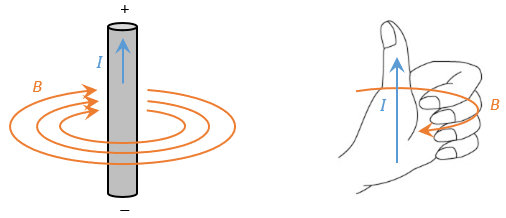
\includegraphics[width=0.7\textwidth]{bilder/MagnetfeldLeiter.png}
    \caption{Magnetfeld im geraden Leiter und Linke-Faust-Regel}
\end{figure}

\subsection{Drahtrahmen im homogenen Magnetfeld}

\end{document}